  \documentclass{beamer}
  \usepackage[utf8]{inputenc}
  \usetheme{Warsaw}
  %\graphicspath{tabularx}
  
  \usepackage{graphicx}
\usepackage{epsfig}
\usepackage{amssymb}
\usepackage{amsmath}
\usepackage{array}
\usepackage{subfig}
\usepackage{multicol}
\usepackage{caption}
\usepackage{listings}
\usepackage{algorithm}
\usepackage{algorithmic}
\usepackage{array,multirow,makecell}

  \title{Stéganographie \& Stéganalyse : Démonstration}
  \author{StegX}
  \institute{UFR des Sciences Versailles - L3 Informatique}
  \date{1er Juin 2018}

  \begin{document}

  \begin{frame}
  \titlepage
  \end{frame}
  
  \section{Ce que propose StegX}
    
	\begin{frame}
  
\includegraphics[scale=0.3]{pictures/bilan_0}
  \end{frame}
  
  \subsection{Interfaces}
  
  \begin{frame}
  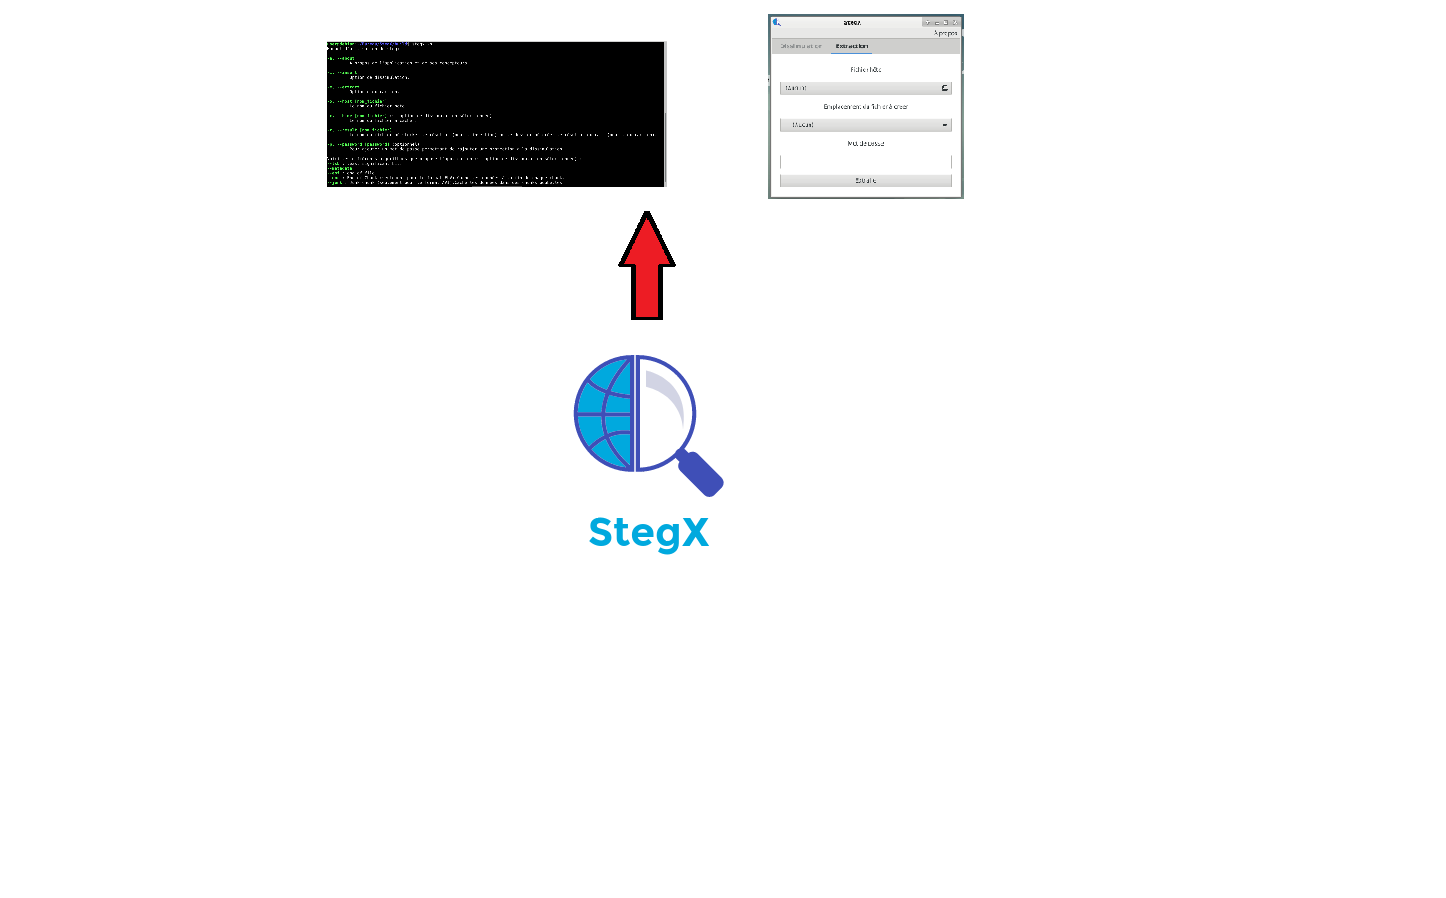
\includegraphics[scale=0.3]{pictures/bilan_1}
  \end{frame}
  
  \subsection{Multi-plateforme}
  
  \begin{frame}
  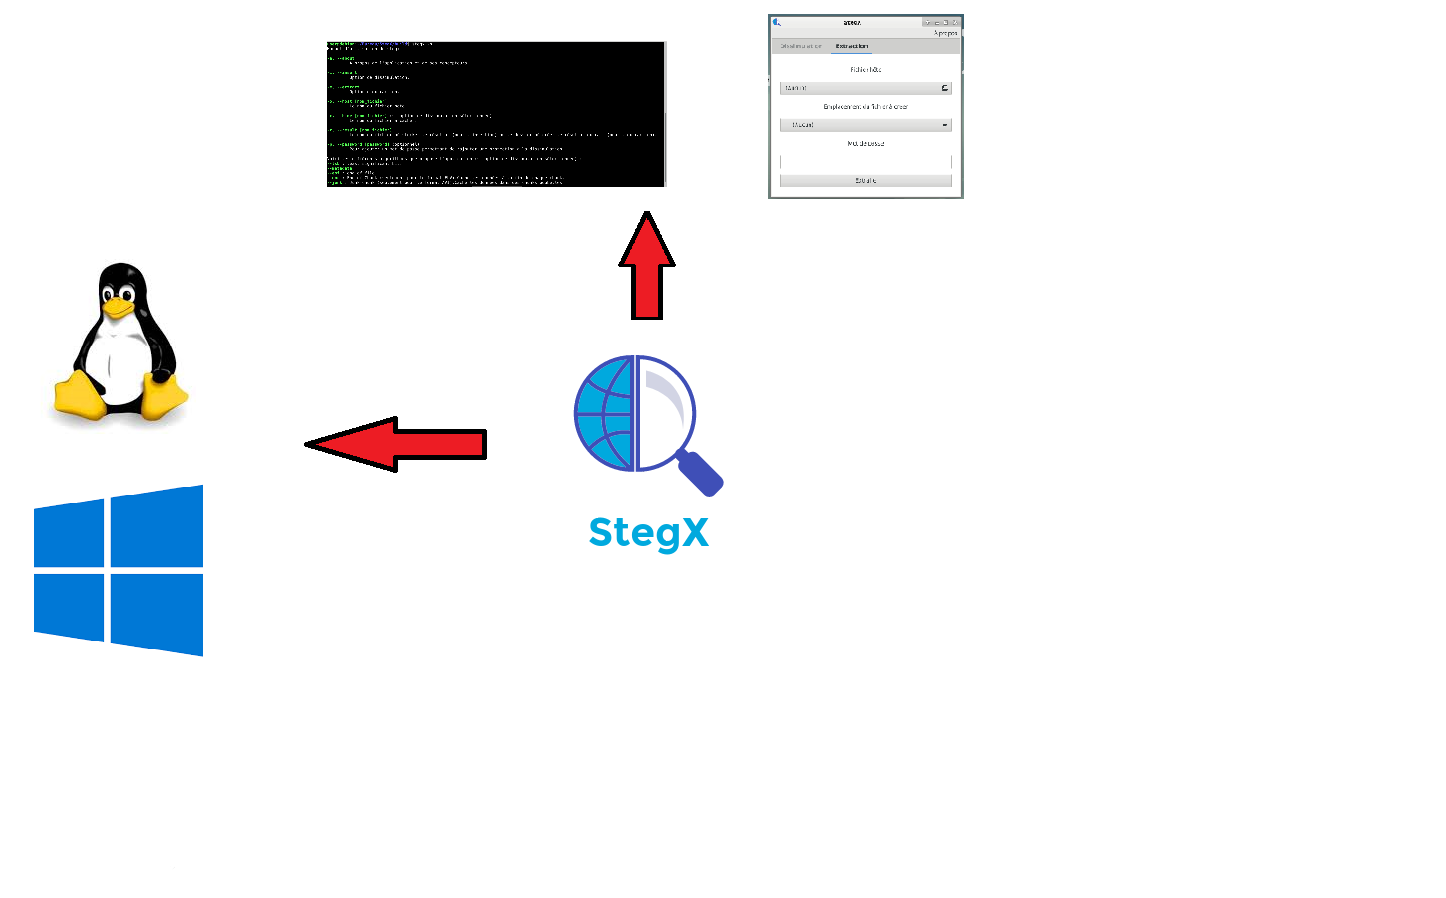
\includegraphics[scale=0.3]{pictures/bilan_2}
  \end{frame}
  
  \subsection{3 types dont 6 formats}
  
  \begin{frame}
  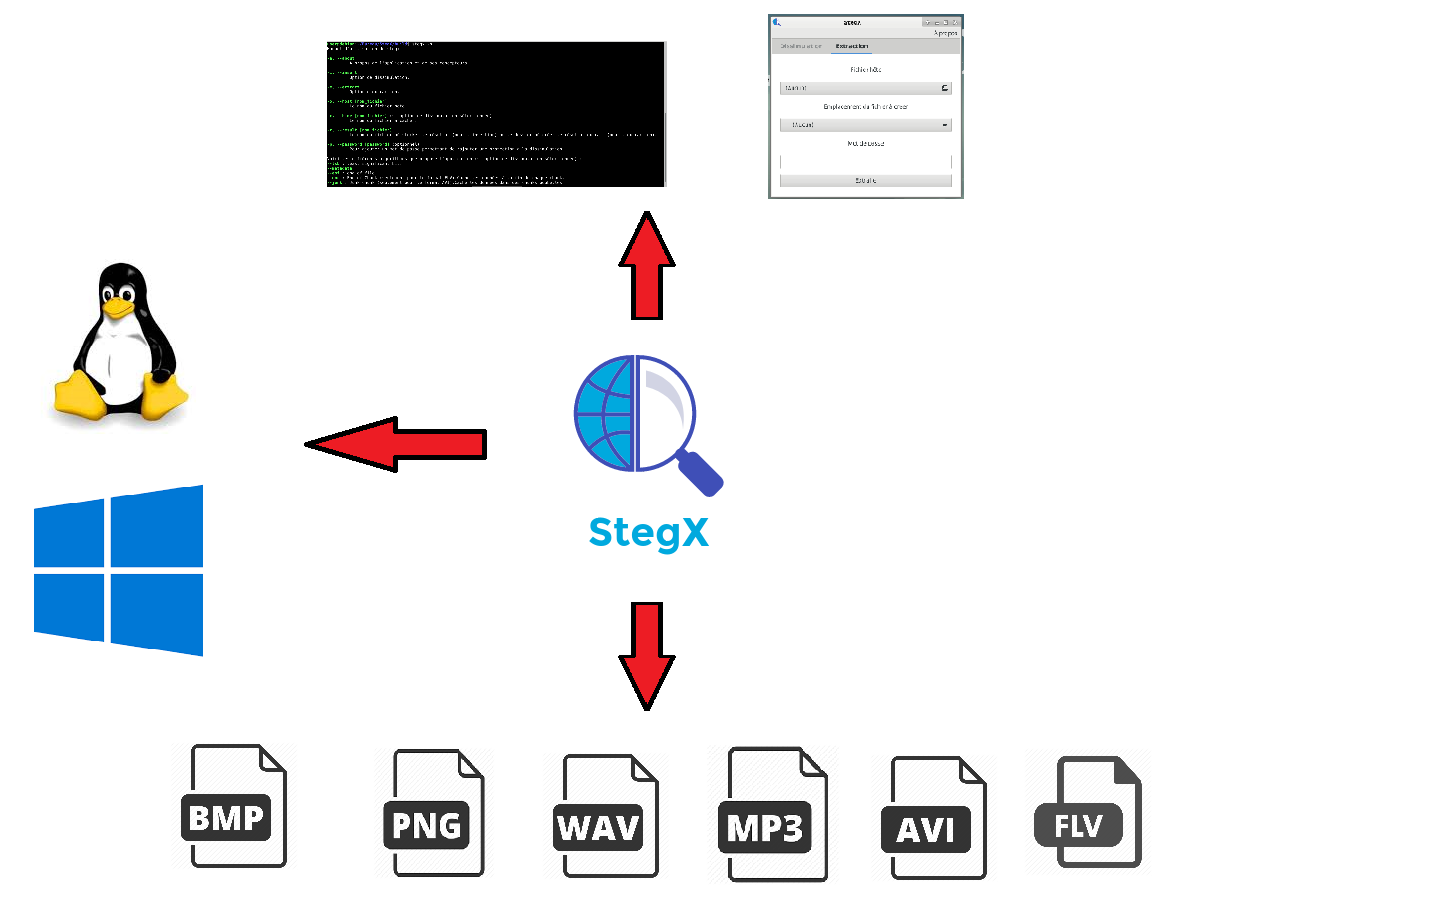
\includegraphics[scale=0.3]{pictures/bilan_3}
  \end{frame}
  
  \subsection{5 algorithmes de stéganographie}
  
  \begin{frame}
  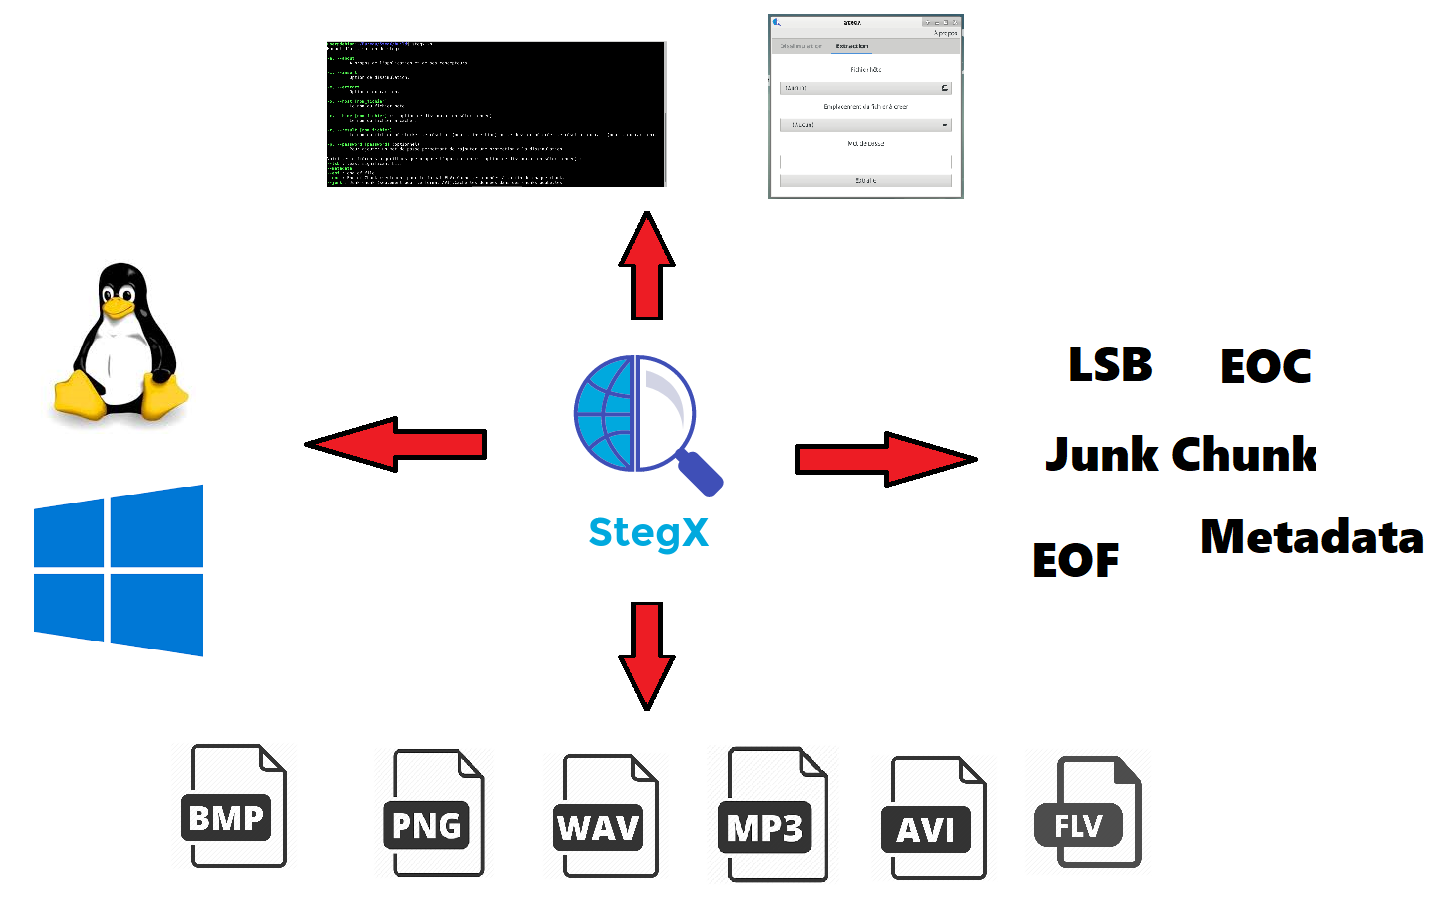
\includegraphics[scale=0.3]{pictures/bilan_4}
  \end{frame}
  
  \section{Introduction et demande du client}
  
  \subsection{Définitions des termes du sujet}
  
  \begin{frame}
  \hspace{5cm}
  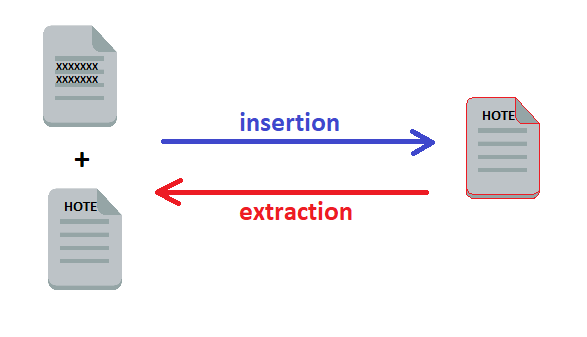
\includegraphics[scale=0.7]{pictures/definition2.png}
  \end{frame}
  
  \subsection{Commande du client}
  
  \begin{frame}
   \begin{block}{Demande du client}
	\begin{itemize}
	\setbeamertemplate{itemize item}[circle]
    \item Cacher des données dans des fichiers
        de type image, audio et vidéo. 
    \item Faire l'extraction automatique des données cachées du 
        fichier à analyser.
    \item Gestion de plusieurs formats et diversité dans les algorithmes proposés.
    \item Proposition d'une bibliothèque partagée par
        deux interfaces différentes, une graphique et une en ligne de commande.
	\end{itemize}
	\end{block}

	Il fallait donc réaliser un logiciel de stéganographie permettant à des
	personnes lambdas de communiquer sans que l'on soupçonne que leurs
	communications soient en réalité compromettantes. 

  \end{frame}
  
  \section{Enchainement des modules}
  \begin{frame}
  \hspace{1.5cm}
  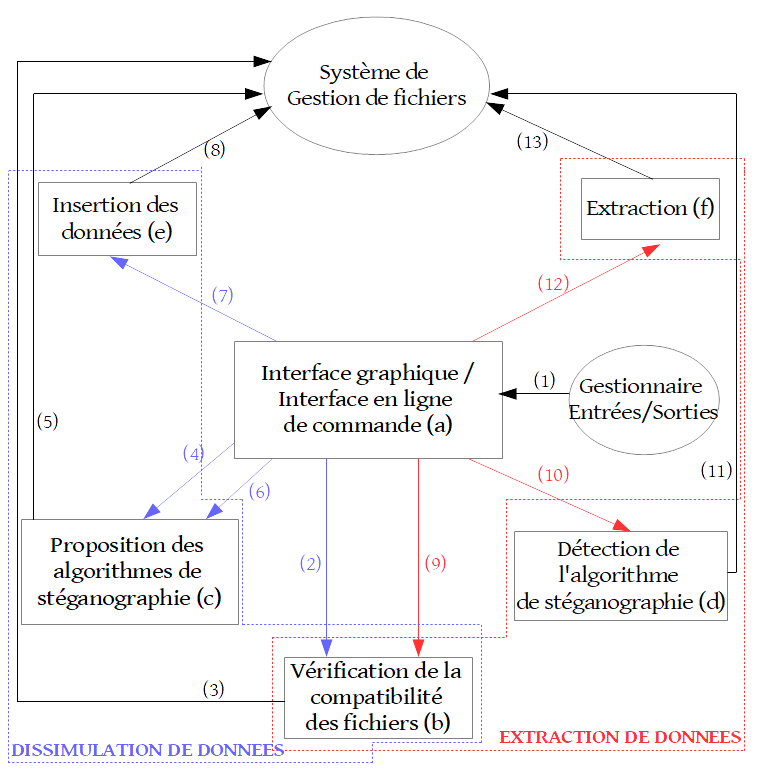
\includegraphics[scale=0.25]{pictures/organigramme_extraction.png}
  \end{frame}
  
  \section{Algorithmes de stéganographie} %OK
  
	% LSB OK
	\subsection{Least Significant Bit (LSB)}
	\begin{frame}
  
	\begin{block}{Least Significant Bit}
	\begin{itemize}
	\setbeamertemplate{itemize item}[circle]
	\item Modification des bits de poids faible des octets de données de 
	l'hôte. 
	\item Proposé pour les formats BMP (non compressé) et WAV (PCM). 
	\end{itemize}
	\end{block}
	
	\hspace{2.5cm}
    
\includegraphics[scale=0.1]{pictures/lsb.png}
	\end{frame}
  
    % EOF OK
    \subsection{End Of File (EOF)}
    \begin{frame}
    
	\begin{block}{End Of File}
	\begin{itemize}
	\setbeamertemplate{itemize item}[circle]
	\item Écriture des données à cacher après la fin officielle du fichier 
	hôte. 
	\item Proposé pour les formats BMP, PNG, WAV et FLV. 
	\end{itemize}
	\end{block}
	
	\hspace{1cm}
    
\includegraphics[scale=0.2]{pictures/eof.png}
    
    \end{frame}
    
    % METADATA OK
	\subsection{Metadata}
    \begin{frame}
    
	\begin{block}{Metadata}
	\begin{itemize}
	\setbeamertemplate{itemize item}[circle]
	\item Écriture des données à cacher dans des blocs de données spécifiques 
	qui ne modifieront pas les données originales. 
	\item Proposé pour les formats BMP et PNG. 
	\end{itemize}
	\end{block}
	
	\hspace{3.5cm}
    
\includegraphics[scale=0.2]{pictures/meta.png}
    
    \end{frame}
    
    %EOC OK
    \subsection{End Of Chunk (EOC)}
    \begin{frame}
    
	\begin{block}{End Of Chunk}
	\begin{itemize}
	\setbeamertemplate{itemize item}[circle]
	\item Écriture des données à cacher après les différents chunks interprétables 
	du fichier hôte. Ces données seront non reconnus et donc ignorés. 
	\item Proposé pour le format FLV.  
	\end{itemize}
	\end{block}
	
	\hspace{4.3cm}
    
\includegraphics[scale=0.08]{pictures/flv_512.png}
    
    \end{frame}
  
	%Junk Chunk OK
    \subsection{Junk Chunk}
    \begin{frame}
    
	\begin{block}{Junk Chunk}
	\begin{itemize}
	\setbeamertemplate{itemize item}[circle]
	\item Écriture des données à cacher dans un chunk appelé "junk" : les 
	données ne seront pas interprétées  
	\item Proposé pour le format AVI. 
	\end{itemize}
	\end{block}
	
	\hspace{4.4cm}
    
\includegraphics[scale=0.08]{pictures/avi-512.png}
    
    \end{frame}

  \section{Conclusion}
  
  \begin{frame}
  
	Le produit répond bien aux objectifs et propose ces algorithmes pour 
	ces formats : 
\newline

\begin{tabular}{|c|c|c|c|c|c|}
  \hline
  \multirow{2}*{\textbf{Format}} & \multicolumn{5}{c|}{\textbf{Algorithmes proposés}} \\
   \cline{2-6}
    & \textbf{LSB} & \textbf{EOF} & \textbf{Metadata} 
    &\textbf{EOC} & \textbf{Junk Chunk} \\
  \hline
  \textbf{BMP} & \textbf{\checkmark} & \textbf{\checkmark} & \textbf{\checkmark} &  & \\
  \hline      
  \textbf{PNG} &  & \textbf{\checkmark} & \textbf{\checkmark} & & \\
  \hline
  \textbf{WAV} & \textbf{\checkmark} & \textbf{\checkmark} & & & \\
  \hline 
  \textbf{MP3} & & \textbf{\checkmark} & & & \\
  \hline 
  \textbf{AVI} & & & & & \textbf{\checkmark}\\
  \hline
  \textbf{FLV} & & \textbf{\checkmark} & & \textbf{\checkmark} & \\
  \hline
\end{tabular}

\end{frame}
  
  \end{document}
  
